\lettrine{C}{on} il termine ``Internet'' ci si riferisce alla rete pubblica formata da dispositivi (nodi) autonomi ed eterogenei distribuiti in tutto il mondo basata su una suite di protocolli standard.

Lo sviluppo di un collegamento tra più nodi è stato motivato originariamente da possibili applicazioni militari, quali collegamenti tra centinaia di università e installazioni governative tramite linee telefoniche.
Per questo motivo la capacità di collegare tra loro diverse reti in maniera semplice è stata sin dall'inizio uno dei principali requisiti di progetto.
Un altro obiettivo era che la rete potesse sopravvivere alla perdita dell'hardware di \textit{subnet} senza interrompere le conversazioni in corso.
Le connessioni dovrebbero rimanere intatte per tutto il tempo in cui il computer sorgente e quello destinazione fossero in funzione, anche se alcuni dei computer o delle linee di trasmissione tra essi fossero andati improvvisamente in avaria.
Inoltre era necessaria un'architettura flessibile, poiché erano previste applicazioni con richieste divergenti, che spaziavano dal trasferimento di file alla trasmissione della voce in tempo reale.
Questi requisiti hanno portato alla scelta di una rete a commutazione di pacchetto basata su uno strato senza connessione.
Il suo scopo è quello di consentire agli host di mandare pacchetti in qualsiasi rete e farli viaggiare in modo indipendente l'uno dall'altro fino alla destinazione.
Potrebbero persino arrivare con un ordine diverso da quello originario e in questo caso (se è richiesta una consegna in sequenza) è compito degli strati superiori ordinarli.
Lo strato internet definisce un formato ufficiale per i pacchetti e un protocollo, il cui scopo è quello di consegnare i pacchetti alla destinazione corretta.
L'instradamento dei pacchetti è chiaramente il problema più importante, assieme alla necessità di garantire l'assenza di congestioni.
Questa architettura è poi diventata nota con il nome del modello di riferimento \verb+TCP/IP+, in funzione dei due più importanti protocolli in essa definiti: il \verb+TCP+ (\textit{Transmission Control Protocol}) e \verb+IP+ (\textit{Internet Protocol}) \cite{TCPIP}.

Su questa architettura, organizzata secondo una logica a livelli sovrapposti, si trovano tutte le applicazioni.
Tuttavia, anche nello strato applicativo c'è l'esigenza di protocolli di supporto che permettono ai software di funzionare.
Nelle successive sezioni verranno introdotti questi protocolli del livello applicativo: \verb+HTTP+ e \verb+MQTT+.

\begin{figure}[H]
  \centering
  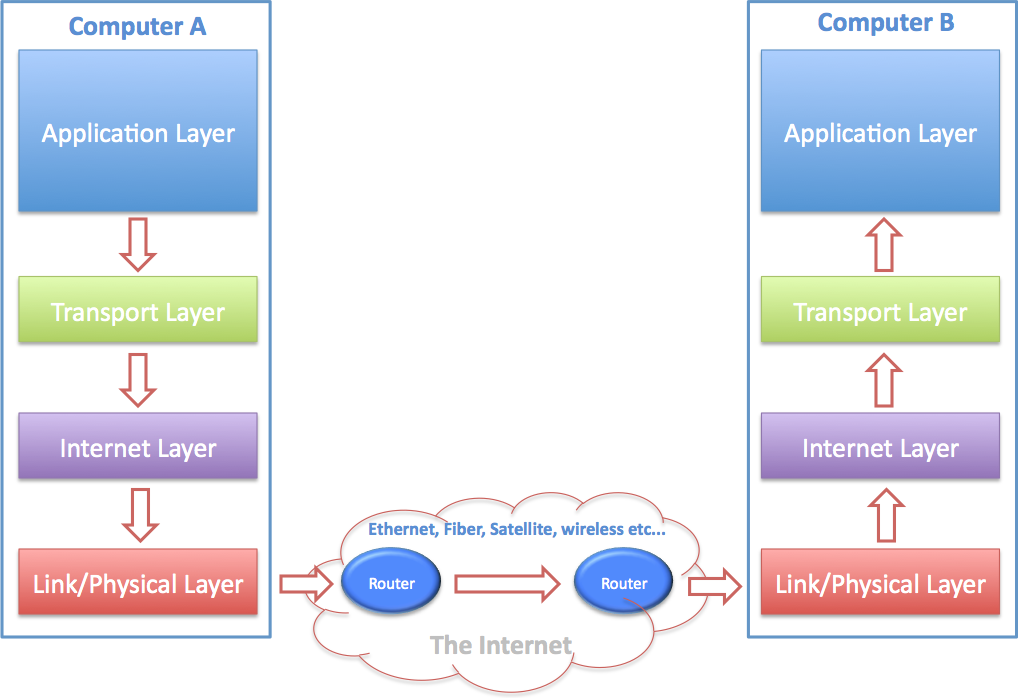
\includegraphics[width=0.95\linewidth, keepaspectratio]{tcpip}
  \caption{Modello dello stack TCP/IP a layer sovrapposti}
  \label{fig:tcpip}
\end{figure}
